% !TEX encoding = IsoLatin2  % notwendige Zeile f"ur Mac-Benutzer (muss als Kommentar stehen); Windos-Benutzer k"onnen die Zeile l"oschen.

% LaTeX-Vorlage Version 3.0,  Juni 2010
% erstellt von Dr. Andreas Drauschke und Dr. Susanne Teschl
% Modifiziert von Dr. Andreas Mehrle (andreas.mehrle@mci.edu)

\documentclass[a4paper,oneside,10pt]{article}%{scrreprt} 
% F"ur kurze Arbeiten w"are auch die Dokumentklasse "scrartcl" ausreichend. In diesem Fall ist "section" die h"ochste Ebene ("chapter" gibt es dann nicht).
% \documentclass[a4paper,bibtotoc,oneside]{scrbook}

\usepackage{ifthen}
\newboolean{english}
%\setboolean{english}{true}		% auskommentieren fuer deutsche Version

\ifthenelse{\boolean{english}}
{}{
	\usepackage{german}
}
\usepackage[dvips]{graphicx}
\usepackage[tmargin=1in,bmargin=1in,lmargin=1.25in,rmargin=1.25in]{geometry}
\usepackage{titlesec}
\usepackage{xcolor}
\usepackage[overload]{textcase}
\definecolor{MSBlue}{rgb}{.204,.353,.541}
\definecolor{MSLightBlue}{rgb}{.31,.506,.741}
% Set formats for each heading level
%\titleformat*{\section}{\rmfamily\bfseries\huge\color{MSBlue}\lowercase}
\titleformat{\section}[hang]{\rmfamily\bfseries\huge\color{MSBlue}\lowercase}{\thesection}{1em}{}[]
\titleformat{\subsection}{\large\bfseries\sffamily\uppercase}{\thesubsection}{1em}{}
\titleformat{\subsubsection}{\sffamily\bfseries}{\thesubsubsection}{1em}{}
\renewcommand\contentsname{\ifthenelse{\boolean{english}}{table of contents.}{inhaltsverzeichnis.}}
\renewcommand\listfigurename{\ifthenelse{\boolean{english}}{list of figures.}{abbildungsverzeichnis.}}
\renewcommand\listtablename{\ifthenelse{\boolean{english}}{list of tables.}{tabellenverzeichnis.}}
\renewcommand\refname{\litname.}
\usepackage{exscale,relsize}
\usepackage{fancyhdr}
\usepackage[small]{caption}
\usepackage{float}
\usepackage{amsmath}
\usepackage{subfigure}
\usepackage{wallpaper}
\usepackage{pst-all}
\usepackage{amssymb}
\usepackage{rotating}
\usepackage[]{amsmath}
\usepackage{mathrsfs}
\usepackage{pgfplots}
\usepackage{makeidx}
%\usepackage[pdftex,bookmarks=true,bookmarksnumbered=true]{hyperref}

\newcommand{\babel}[2]{\ifthenelse{\boolean{english}}{#1}{#2}}

% color set
\definecolorseries{foo}{rgb}{last}[rgb]{1.0,0.0,0.0}[rgb]{0.0,0.0,1.0}
\resetcolorseries[16]{foo}

% auxillary symbols
\renewcommand{\tilde}{\symbol{126}}
\newcommand{\define}{\stackrel{!}{=}}
\renewcommand{\equiv}{\,\widehat{=}\,}
\newcommand{\subsubsubsection}{\textbf}
\newcommand{\re}{\mathrm{Re}}
\newcommand{\pr}{\mathrm{Pr}}
\newcommand{\st}{\mathrm{St}}
\newcommand{\fr}{\mathrm{Fr}}
\newcommand{\nus}{\mathrm{Nu}}
\newcommand{\gr}{\mathrm{Gr}}
\newcommand{\ra}{\mathrm{Ra}}
\newcommand{\mif}{\quad\mathrm{\babel{if}{falls}}\quad}
\newcommand{\with}{\quad\mathrm{\babel{with}{mit}}\quad}
\newcommand{\for}{\quad\mathrm{\babel{for}{f"ur}}\quad}
%\renewcommand{\not}{\not}
\newcommand{\im}{i}
\newcommand{\ariwam}{ARiWaM}
\newcommand{\matlab}{MATLAB}

% format specifications
\renewcommand{\emph}{\textbf}
\newcommand{\file}{\textit}
\newcommand{\cmd}{\texttt}
\newcommand{\ten}{\boldsymbol}
%\newcommand{\unit}{\mathrm}
\newcommand{\lemma}{\textit}
\newcommand{\deutsch}[1]{german: \textit{#1}}
\renewcommand{\index}{\emph}

% Command path to graphic files
\newcommand{\gpath}{./grafics}
\newcommand{\bsppath}{../uebungen/beispiele}

% mathematical operators
\newcommand{\grad}{\,\mathrm{grad}\,}
\renewcommand{\div}{\,\mathrm{div}\,}
\newcommand{\rot}{\,\mathrm{rot}\,}
\newcommand{\lap}{\Delta}
\newcommand{\laplace}[1]{\mathscr{L}\left\{#1\right\}}
\newcommand{\trans}{^T}
\newcommand{\norm}{\psarc[linewidth=0.5pt](0,0){0.4}{0}{90}\psdot[dotsize=0.1](0.15,0.15)}

% electrical networks
\newcommand{\con}{\pscircle[linewidth=2pt,fillstyle=solid,fillcolor=black](0,0){0.1}}
\newcommand{\pin}{\pscircle[linewidth=2pt,fillstyle=solid](0,0){0.15}}
\newcommand{\link}{\psline[linewidth=2pt]}
\newcommand{\linkd}{\psline[linestyle=dashed]}
\newcommand{\arcd}{\psarc[linestyle=dashed]}
\newcommand{\arrow}{\psline[linewidth=2pt,arrowsize=8pt]{->}}
\newcommand{\cs}{\pscircle[linewidth=2pt](0,0){0.5}\arrow(0,-0.4)(0,0.4)\link(0,-0.5)(0,-2)\link(0,0.5)(0,2)}
\newcommand{\vs}{\pscircle[linewidth=2pt](0,0){0.5}\psline(-0.2,-0.1)(0.2,-0.1)\psline(-0.2,0)(0.2,0)\pscurve(-0.2,0.1)(-0.1,0.15)(0,0.1)(0.1,0.05)(0.2,0.1)\link(0,-0.5)(0,-2)\link(0,0.5)(0,2)}
\newcommand{\res}{\psframe[linewidth=2pt](-0.3,-1)(0.3,1)\link(0,-1)(0,-2)\link(0,1)(0,2)}
\newcommand{\ind}{\psframe[linewidth=2pt,fillstyle=solid,fillcolor=black](-0.3,-1)(0.3,1)\link(0,-1)(0,-2)\link(0,1)(0,2)}
\renewcommand{\cap}{\link(-0.5,-0.1)(0.5,-0.1)\link(-0.5,0.1)(0.5,0.1)\link(0,-0.1)(0,-2)\link(0,0.1)(0,2)}
\newcommand{\opv}{\pspolygon[linewidth=2pt](-1,-1.3)(-1,1.3)(1.3,0)\link(-1,-0.8)(-2,-0.8)\link(-1,0.8)(-2,0.8)\link(1.3,0)(2,0)\rput(-0.7,0.8){$-$}\rput(-0.7,-0.8){$+$}}

% mechanical networks
\newcommand{\mass}{\psframe[linewidth=2pt](-0.5,-0.5)(0.5,0.5)\link(0,0.5)(0,1)\link(0,-0.5)(0,-1)}
\newcommand{\spring}{\link(0,-1)(0,-0.8)(-0.3,-0.7)(0.3,-0.5)(-0.3,-0.3)(0.3,-0.1)(-0.3,0.1)(0.3,0.3)(-0.3,0.5)(0.3,0.7)(0,0.8)(0,1)}
\newcommand{\damp}{\link(-0.5,0.4)(-0.5,-0.3)(0.5,-0.3)(0.5,0.4)\link(-0.42,0.2)(0.42,0.2)\link(0,0.2)(0,1)\link(0,-0.3)(0,-1)}
\newcommand{\hatch}{\psframe[fillstyle=vlines,linestyle=none,hatchwidth=0.25pt]}
\newcommand{\clamp}{\hatch(-0.5,-0.3)(0.5,0)\link(-0.5,0)(0.5,0)}
\newcommand{\fixed}{\hatch(-0.5,-0.7)(0.5,-0.4)\link(-0.5,-0.4)(0.5,-0.4)\link(-0.25,-0.4)(0,0)(0.25,-0.4)\pscircle[linewidth=2pt,fillstyle=solid](0,0){0.1}}
\newcommand{\loose}{\hatch(-0.5,-0.7)(0.5,-0.5)\link(-0.5,-0.4)(0.5,-0.4)\link(-0.5,-0.5)(0.5,-0.5)\link(-0.25,-0.4)(0,0)(0.25,-0.4)\pscircle[linewidth=2pt,fillstyle=solid](0,0){0.1}}
\newcommand{\axial}{\link(-0.3,-0.3)(-0.3,-0.1)(0.3,-0.1)(0.3,-0.3)\link(-0.3,0.3)(-0.3,0.1)(0.3,0.1)(0.3,0.3)}
\newcommand{\force}{\psline[linewidth=2pt,arrowsize=6pt]{->}}
\newcommand{\rmom}{\psarc[arrowsize=6pt,linewidth=2pt]{<-}}
\newcommand{\lmom}{\psarc[arrowsize=6pt,linewidth=2pt]{->}}
\newcommand{\stress}{\psline[arrowsize=6pt]{->}}
\newcommand{\beam}{\psframe[fillstyle=solid,fillcolor=lightgray]}
\newcommand{\rod}{\psline[linewidth=3pt]}
\newcommand{\disp}{\psline[linewidth=2pt,arrowsize=6pt]{->}}	% displacement

% hydraulical networks
\newcommand{\pump}{\pscircle[linewidth=2pt,fillstyle=solid,fillcolor=white](0,0){1}\pspolygon[fillstyle=solid,fillcolor=black](0,1)(-0.15,0.3)(0.15,0.3)}
\newcommand{\motor}{\pscircle[linewidth=2pt,fillstyle=solid,fillcolor=white](0,0){0.8}\rput(0,0){M}}
\newcommand{\throttle}{\psarc[linewidth=2pt](-3,0){2.7}{-15}{15}\psarc[linewidth=2pt](3,0){2.7}{165}{195}}
\newcommand{\limiter}{\psframe[linewidth=2pt,fillstyle=solid,fillcolor=white](-0.7,-0.7)(0.7,0.7)\psline{->}(-0.5,-0.4)(-0.5,0.1)(0.5,-0.25)}

% diagrams (block and s-plane)
\newcommand{\axis}{\psline[arrowsize=6pt,arrowinset=0]{->}}
\newcommand{\measure}{\psline[linewidth=0.5pt,arrowsize=4pt]}
\newcommand{\xtick}[1]{\measure(#1,-0.1)(#1,0.1)}
\newcommand{\ytick}[1]{\measure(-0.1,#1)(0.1,#1)}
\newcommand{\angarc}{\psarc[linewidth=0.5pt,arrowsize=4pt]{<->}}
\newcommand{\tf}[1]{\psframe[linewidth=2pt](-1,-0.75)(1,0.75)\rput(0,0){#1}}
\newcommand{\tff}[2]{\psframe[fillstyle=solid,fillcolor=lightgray](-1,0)(1,0.75)\psframe[linewidth=2pt](-1,-0.75)(1,0.75)\rput(0,0.35){#1}\rput(0,-0.35){#2}}
\newcommand{\sat}{\psframe[linewidth=2pt](-1,-0.75)(1,0.75)\link(-0.8,-0.5)(-0.5,-0.5)(0.5,0.5)(0.8,0.5)}
\newcommand{\add}[4]{\pscircle[linewidth=2pt,fillstyle=solid,fillcolor=white](0,0){0.5}\rput(-0.5,-0.75){#1}\rput(-0.75,0.5){#2}\rput(0.5,0.75){#3}\rput(0.75,-0.5){#4}}
\newcommand{\pole}{\link(-0.15,-0.15)(0.15,0.15)\link(-0.15,0.15)(0.15,-0.15)}
\newcommand{\zero}{\pscircle[linewidth=2pt,fillstyle=solid](0,0){0.15}}
\newcommand{\textblock}[1]{\psframebox[linewidth=2pt]{\parbox[c][2cm][c]{3cm}{\centering #1}}}

% thermodynamic systems
\newcommand{\cv}{\psframe[linestyle=dashed]}
\newcommand{\sys}{\psframe[fillcolor=white,fillstyle=solid,linewidth=2pt]}
\newcommand{\iso}{\psframe[linewidth=2pt,fillstyle=vlines]}
\newcommand{\candle}{\psframe[linewidth=0.5pt](-0.15,-0.5)(0.15,0.3)\pscurve[linewidth=0.5pt](0,0.8)(-0.1,0.5)(0,0.3)(0.1,0.5)(0,0.8)\pscurve[linewidth=0.5pt](0,0.6)(-0.08,0.4)(0,0.3)(0.08,0.4)(0,0.6)}
\newcommand{\flux}{\psline[arrowsize=10pt,linewidth=4pt]{->}}
\newcommand{\point}[1]{\pscircle(0,0){0.3}\rput[c](0,0){#1}}

% aerodynamics
\newcommand{\source}{\pin\rput{0}(0,0){\arrow(0.5,0)(1,0)}\rput{45}(0,0){\arrow(0.5,0)(1,0)}\rput{90}(0,0){\arrow(0.5,0)(1,0)}\rput{135}(0,0){\arrow(0.5,0)(1,0)}\rput{180}(0,0){\arrow(0.5,0)(1,0)}\rput{225}(0,0){\arrow(0.5,0)(1,0)}\rput{270}(0,0){\arrow(0.5,0)(1,0)}\rput{315}(0,0){\arrow(0.5,0)(1,0)}}

% CFD
\newcommand{\cell}[1]{\definecolor{cellc}{gray}{#1}\psframe[linewidth=2pt,fillstyle=solid,fillcolor=cellc](0,0)(1,1)}

%\renewcommand{\labelenumi}{\alph{enumi})}

\setlength{\parindent}{0em}
\setlength{\parskip}{1.5ex plus0.5ex minus0.5ex}
\setlength{\captionmargin}{3em}

% counters
\newcounter{example}
\ifthenelse{\boolean{english}}{\newcommand{\exampletext}{example }}{\newcommand{\exampletext}{Beispiel }}
\newcommand{\example}[1]{\underline{\exampletext \arabic{chapter}.\arabic{example}:} #1 \addtocounter{example}{1}}
\newcounter{exercise}
\ifthenelse{\boolean{english}}{\newcommand{\exercisetext}{exercise }}{\newcommand{\exercisetext}{Aufgabe }}
\newcommand{\exercise}[1]{\underline{\exercisetext \arabic{chapter}.\arabic{exercise}:} #1 \stepcounter{exercise}}
\newcommand{\cchapter}[1]{\chapter{#1} \setcounter{example}{1} \setcounter{exercise}{1}}
\ifthenelse{\boolean{english}}{\newcommand{\solution}{\textit{solution:} }}{\newcommand{\solution}{\textit{L\"osung:} }}
%\newcounter{beispiel}
%\setcounter{beispiel}{1}		% Nummer des ersten Beispiels
\newboolean{student}
\newcounter{enumcount}
\newcommand{\resume}[1]{\begin{#1} \setcounter{enumi}{\value{enumcount}}}
\newcommand{\pause}[1]{\setcounter{enumcount}{\value{enumi}} \end{#1}}




\def\labtitle{Biosignalverarbeitung}
\def\labcode{MGST-B-3-BB-BS-ILV}
\def\labname{Aufbau der Hardware und Datenakquise}
\def\labnum{1}

\def\study{Bachelor Medizin-, Gesundheits- und Sporttechnologien}
\def\term{3.}
\def\lecturer{Dr. Gerda Strutzenberger, Aitor Morillo}
\def\group{MGST-BA-25-VZ}
\def\student{Julius Weber, Jannis Hammerer, Matthias Winter}

\def\litname{literatur}

\begin{document}

%\layout

% Kopf- und Fusszeilen initiieren
\pagestyle{plain}

% Deckblatt:
\thispagestyle{empty}
\sffamily
%\put(-30,-685){\includegraphics[width=1.15\linewidth]{BG}}

{\bfseries


\vspace*{1cm}

\def\thesis{\ifthenelse{\boolean{english}}{laboratory report}{laborbericht}}
\textcolor{MSBlue}{\rmfamily\bfseries\huge\thesis.}%

\vspace*{0.5cm}

\textbf{\labtitle{ }(\labcode)}

\labname

\ifthenelse{\boolean{english}}{Lab}{Labor} \labnum

\vspace*{10cm}

\textcolor{gray}{\study}

\def\termname{\ifthenelse{\boolean{english}}{semester}{Semester}}
\textcolor{gray}{\term{ }\termname}

\def\lecturername{\ifthenelse{\boolean{english}}{Responsible lecturer}{Lehrveranstaltungsleiter}}
\textcolor{gray}{\lecturername: \lecturer}

\def\groupname{\ifthenelse{\boolean{english}}{Group}{Jahrgang}}
\textcolor{gray}{\groupname: \group}

\def\authorname{\ifthenelse{\boolean{english}}{Author}{Verfasser}}
\textcolor{gray}{\authorname: \student}

\textcolor{gray}{\today}

\newpage}


\tableofcontents%\thispagestyle{empty}
\listoffigures
\listoftables

\newpage

% Kopf- und Fusszeilen initiieren
\pagestyle{fancy}

\section{Einleitung}

Dieses Dokument stellt eine Vorlage zur Erstellung von Laborberichten in \LaTeX f"ur den Studiengang Mechatronik dar. Achten Sie darauf, dass Sie die jeweils aktuellste Version verwenden. Richtlinien k"onnen sich von Jahr zu Jahr "andern.

\section{Versuchsbeschreibung}

% Aufgabe 1: Aufbau des Messsystems (MMA8452Q + Qwiic OpenLog)
% In der vorhandenen Uni-Vorlage unter \section{Versuchsbeschreibung} einbinden.
% Voraussetzung: abbildungen/messsystem_aufgabe1.eps

\subsection{Messsystem -- Aufgabe 1}

Abbildung~\ref{fig:messsystem} zeigt den schematischen Aufbau des Messsystems
zur Erfassung und Speicherung von Beschleunigungsdaten.

\begin{figure}[htbp]
    \centering
    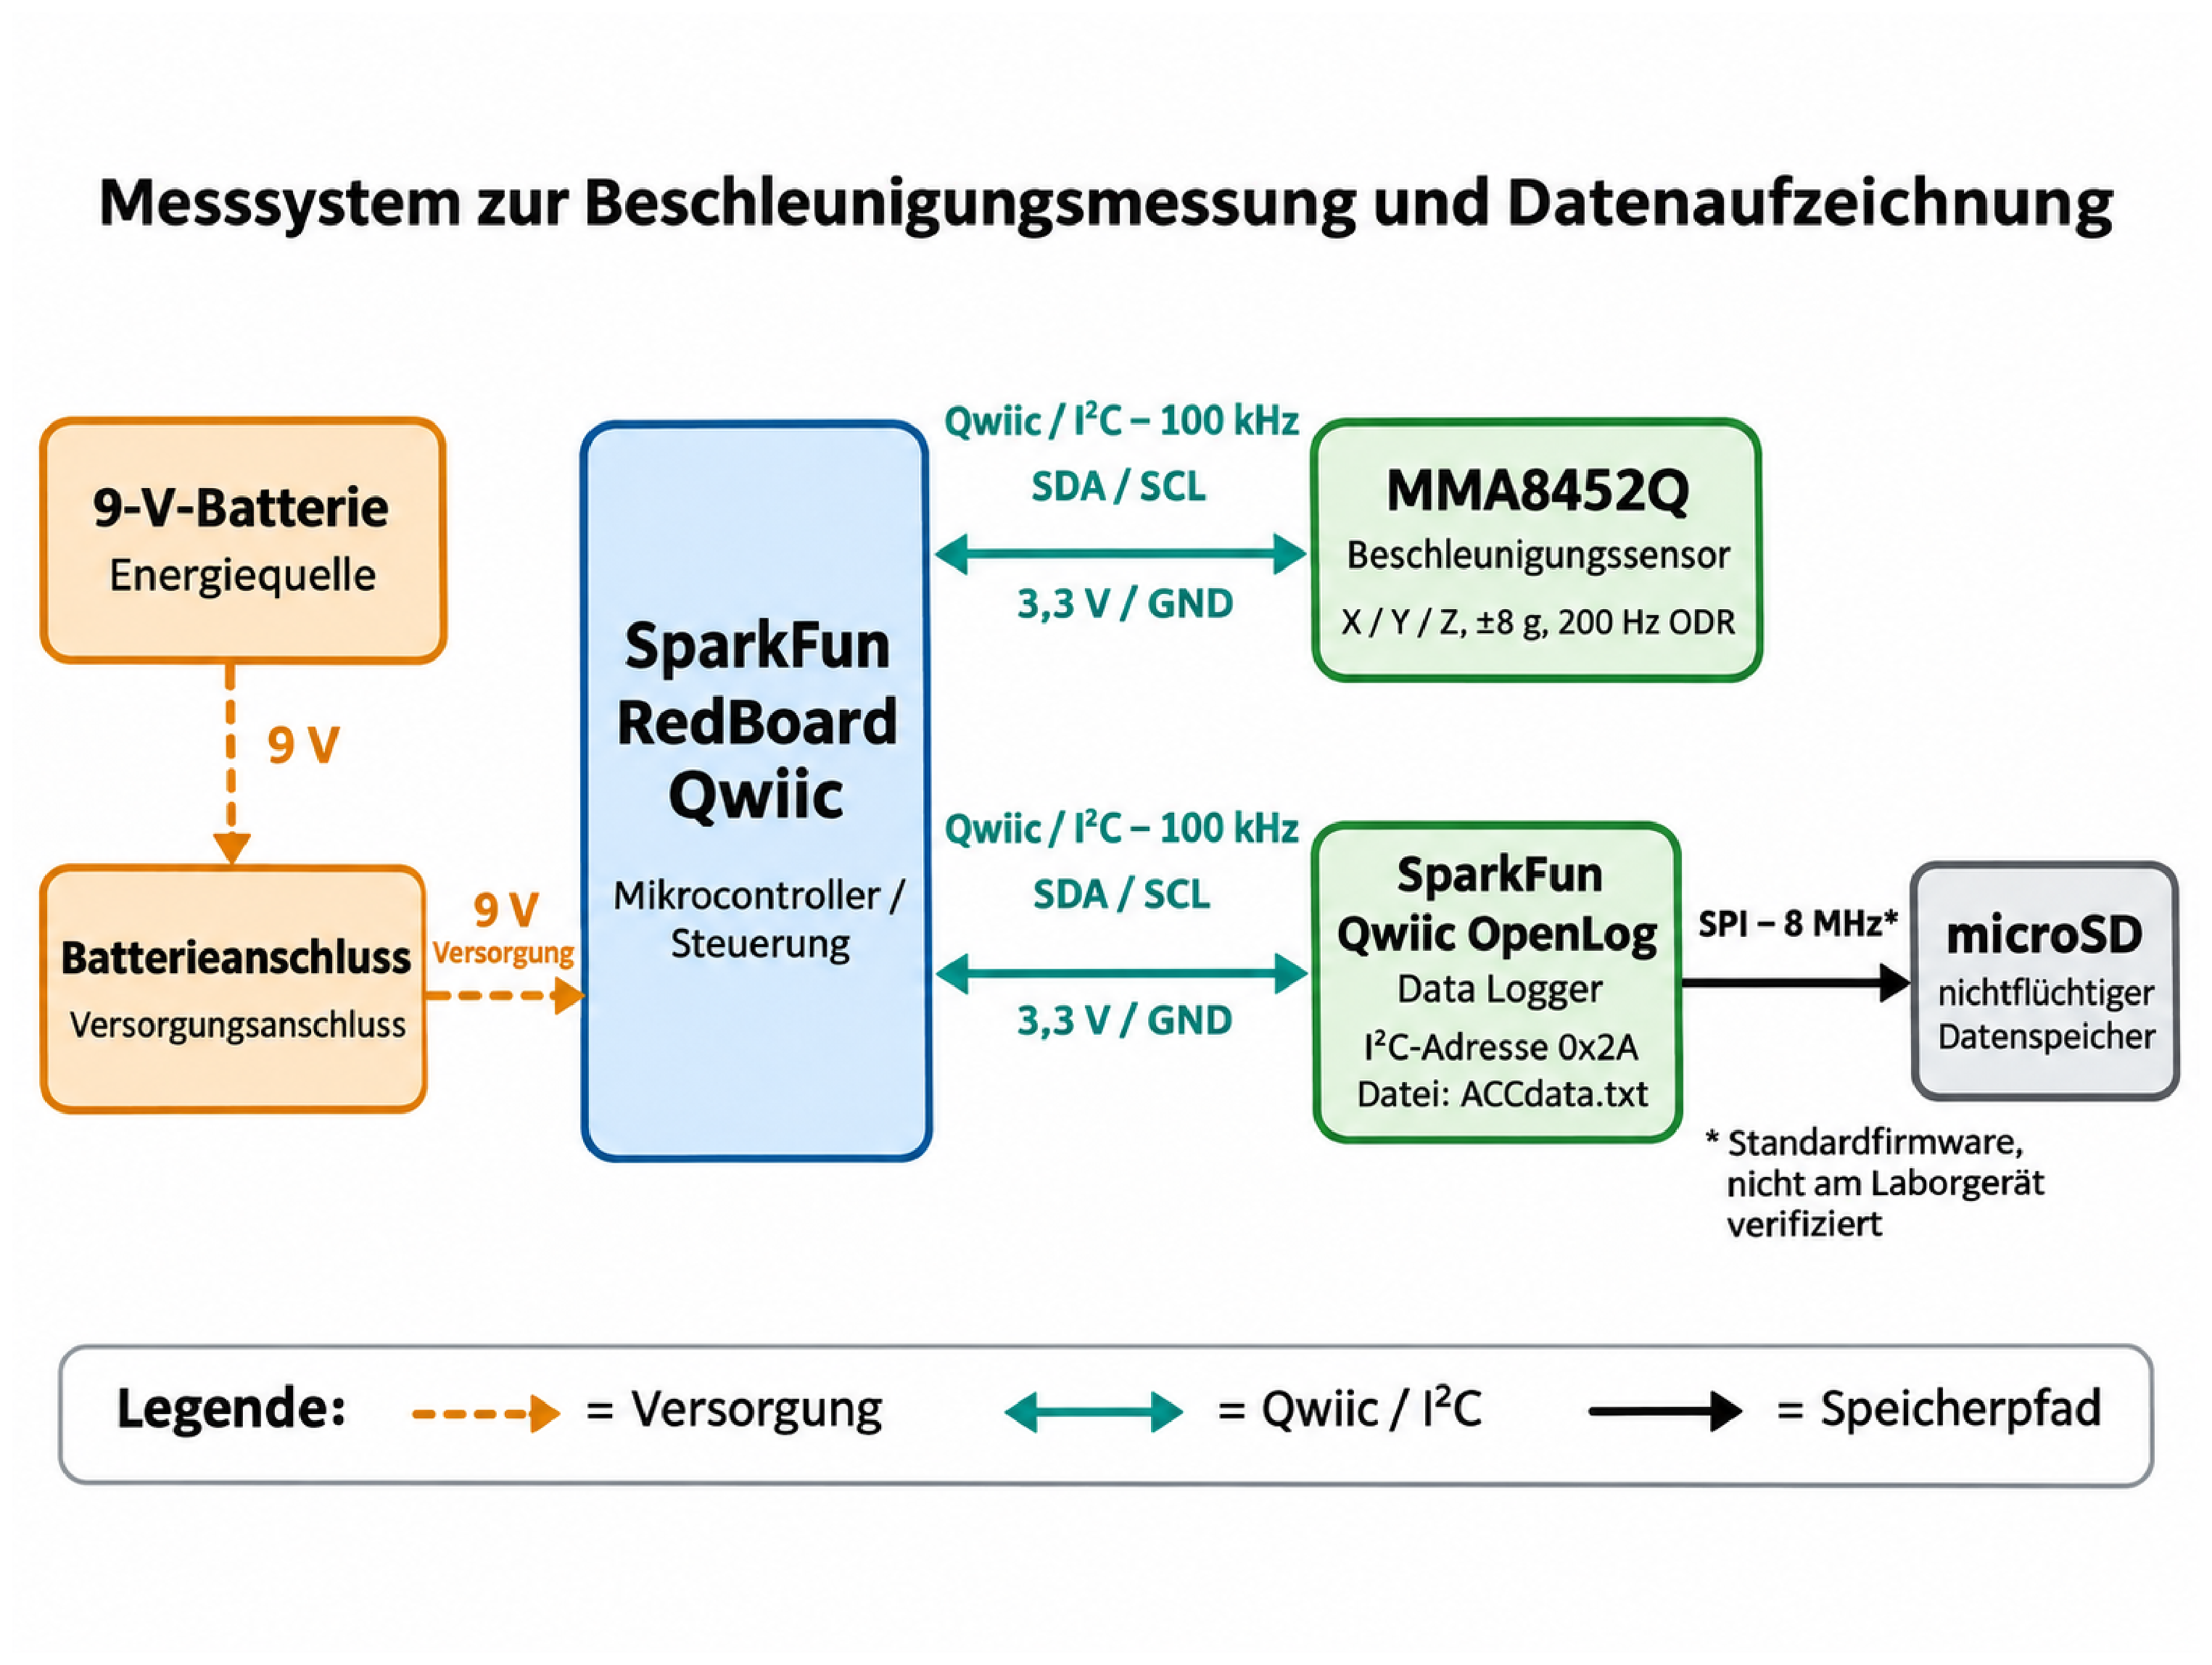
\includegraphics[width=\linewidth,keepaspectratio]{abbildungen/messsystem_aufgabe1_neu.eps}
    \caption{Blockschaltbild des Messsystems zur Beschleunigungsmessung und
    Datenaufzeichnung (eigene Darstellung; SPI-Takt nach Standardfirmware).}
    \label{fig:messsystem}
\end{figure}

\textbf{9-V-Batterie:}
Die Batterie stellt die externe elektrische Energie f\"ur das Messsystem bereit.

\textbf{Batterieanschluss:}
Der Anschluss verbindet die 9-V-Batterie mit dem vorgesehenen
Versorgungseingang des SparkFun RedBoards.

\textbf{SparkFun RedBoard Qwiic:}
Das RedBoard steuert die Messung, liest die Beschleunigungswerte des Sensors
aus und \"ubermittelt sie an den Data Logger. Die Kommunikation mit beiden
Qwiic-Modulen erfolgt \"uber I$^2$C (SDA/SCL) mit einem Standardtakt von
100\,kHz; die Module werden \"uber den Qwiic-Anschluss mit 3,3\,V und GND versorgt.

\textbf{MMA8452Q-Beschleunigungssensor:}
Der Sensor erfasst die Beschleunigungen entlang der drei Achsen X, Y und Z.
Im bereitgestellten Arduino-Programm zur Datenaufzeichnung mit dem Qwiic
OpenLog sind ein Messbereich von $\pm 8\,\mathrm{g}$ und eine Sensordatenrate
(ODR) von $200\,\mathrm{Hz}$ eingestellt.

\textbf{SparkFun Qwiic OpenLog:}
Der Data Logger empf\"angt die vom RedBoard \"ubertragenen Messwerte \"uber
den I$^2$C-Bus (Standardadresse \texttt{0x2A}) und zeichnet sie in der Datei
\texttt{ACCdata.txt} auf der microSD-Karte auf.

\textbf{microSD-Karte:}
Die Speicherkarte dient als nichtfl\"uchtiger Datenspeicher und ist im
OpenLog eingesteckt. Ihre interne Anbindung erfolgt \"uber SPI; die in der
Grafik genannten 8\,MHz beziehen sich auf die Standardfirmware und wurden
am Laborger\"at nicht eigens verifiziert.

\clearpage
\subsection{Temperaturbestimmung -- Aufgabe 2}

Gegeben sind ein ADC-Messwert von $N=520$, eine Aufl\"osung von
$n=10\,\mathrm{Bit}$ und eine maximale ADC-Eingangsspannung von
$U_{\mathrm{ADC,max}}=5\,\mathrm{V}$. Der lineare Temperatursensor liefert bei
$T_{\max}=40\,^\circ\mathrm{C}$ eine Spannung von
$U_{\mathrm{Sensor,max}}=3{,}3\,\mathrm{V}$. Gesucht ist die zum Messwert
geh\"orende Temperatur $T$.

Zun\"achst wird der ADC-Messwert in eine Eingangsspannung umgerechnet. Ein
$n$-Bit-ADC besitzt $2^n$ Abstufungen; der gr\"o{\ss}te darstellbare Messwert
ist daher $N_{\max}=2^n-1$. Anschlie{\ss}end wird die Spannung anhand der
linearen Kennlinie des Sensors in eine Temperatur umgerechnet:

\begin{align*}
N_{\max}
    &= 2^n - 1
     = 2^{10} - 1
     = 1023, \\
U_{\mathrm{Sensor}}
    &= \frac{N}{N_{\max}}\,U_{\mathrm{ADC,max}} \\
    &= \frac{520}{1023}\cdot 5\,\mathrm{V}
     = 2{,}5415\,\mathrm{V}
     \approx 2{,}54\,\mathrm{V}, \\
T
    &= \frac{U_{\mathrm{Sensor}}}{U_{\mathrm{Sensor,max}}}\,T_{\max} \\
    &= \frac{2{,}5415\,\mathrm{V}}{3{,}3\,\mathrm{V}}
       \cdot 40\,^\circ\mathrm{C}
     = 30{,}806\ldots\,^\circ\mathrm{C}
     \approx 30{,}8\,^\circ\mathrm{C}.
\end{align*}

\noindent\textbf{Ergebnis:}
\[
    \boxed{T \approx 30{,}8\,^\circ\mathrm{C}}
\]
Der ADC-Messwert 520 entspricht somit einer Temperatur von etwa
$30{,}8\,^\circ\mathrm{C}$.


\section{Vorausgehende Arbeiten}

Normalerweise sind Sie dazu angehalten sich auf die Labor"ubungvorzubereiten. Diese Arbeit ist f"ur das Verst"andnis ihres Berichtes essentiell und sollte ebenfalls der eigentlichen Labordokumentation vorangestellt werden. Im Speziellen betrifft dies
\begin{itemize}
\item die Messstrategie
\item allf"allige Berechnungen und Absch"atzungen
\item von Ihnen angefertigte Skripte (Quellcode in den Anhang)
\item vorab get"atigte Simulationen
\end{itemize}
Vergessen Sie nicht verwendete Literatur zu zitieren wie z.B.~Skripten, siehe \cite{meh10}.

\section{Grafische Darstellung der Ergebnisse}

Bzgl.~der grafischen Darstellung der Ergebnisse beachten Sie den diesbez"uglichen Leitfaden. Hier noch in K"urze due h"aufigsten Probleme aufgez"ahlt
\begin{itemize}
\item Jeder Graph muss vom Text referenziert werden. Falls nicht stellt dies seine Notwendigkeit in Frage.
\item Kurven m"ussen auch nach einer schwarz-wei"s-Kopie unterscheidbar bleiben. Dies geschieht am besten durch Unterschiede im Linienstil (durchgezogen, strichliert, punktiert, $\ldots$).
\item Werden mehrere Kurven in einen Graphen eingetragen, so ist entweder eine Legende einzuf"ugen (ab 3 Kurven) oder diese in der Bildunterschrift zu unterscheiden (2 Kurven).
\item Die Achsen m"ussen beschriftet werden (\textit{Symbol}/Einheit).
\item Schwarzer Hintergrund ist nicht zul"assig!
\end{itemize}

\bibliographystyle{IEEEtran}	
\bibliography{Literatur}

\end{document}
